






% =========----------	[ Space left here for distraction free mode] ----------==========%









\subsection{Analysis 2: Does the choice of microphone array affect Spatial Attribute score?}
	\label{ana2}


		Breaking down the data showing in figure~\ref{image:AvsB}, the average spatial attribute score across all used microphone configurations is shown in figure~\ref{image:sa_allmics}. The Anderson-Darling test was used to determine that not all of the sample data (participants scores per microphone) is normally distributed. Due to non-normally distributed data the Kurskal-Wallis (K-W) ANOVA was used to determine whether the average scores between any of the samples were significantly different. All groups returned $p > 0.05 $ other than 'Sense of Space' which returned $p = 0.0227 $. As determined in section~\ref{ana1} there is no statistically significant difference between the data due to different viewing positions A and B. Therefore the data was separated according to their viewing positions and another K-W test was conducted on each group. This indicated a significant difference within the group of data from viewing position B, returning $ p = 0.0035 $.

		Using MATLABs \textit{multcompare} function, a post-hoc test was conducted to determine that the sample data for two microphone arrays, OCT and Hamasaki Cube are significantly different to the sample data for the spot microphones, circled in red and blue respectively in figure~\ref{image:sa_allmics}.\\

		\textbf{Conclusion} \\

		 Looking at the scores for the OCT and Hamasaki cube across all spatial attributes, it is apparent that they typically perform well among other microphone configurations. It is therefore probably more appropriate to look at this result as a significantly poor performance from the spot microphones whilst compared to microphone arrays that consistently perform well as opposed to an significantly exceptional performance from the two microphone arrays. Across all other spatial attributes it has been shown that the difference between performance is not statistically significant.

		\begin{figure*}
			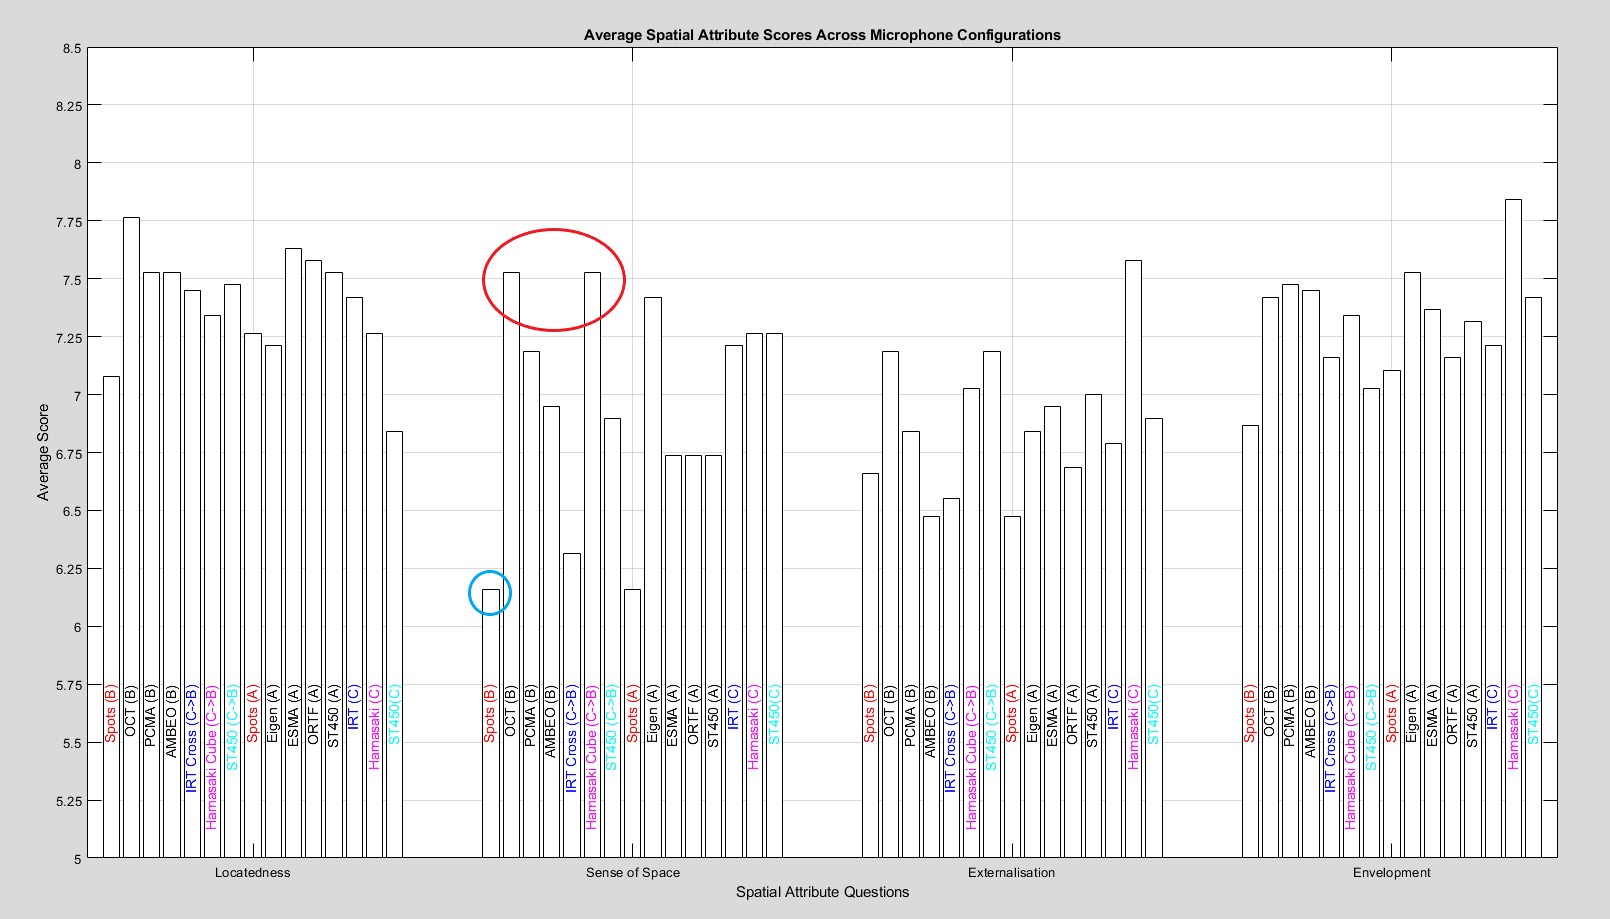
\includegraphics[width=1\textwidth]{images/plots/allMics_edit.PNG}
			\caption{Bar chart of the average spatial attribute score across all microphone configurations where \textit{microphone(X)} indicates the microphone configuration and location. The microphone names are displayed on their corresponding bar where (C$->$B) indicates a microphone from position C whilst viewing from B and (C) indicates a microphone from position C whilst viewing from position A. Microphones that were shared across both viewing positions are highlighted in matching colours.}
			\label{image:sa_allmics} 
		\end{figure*}